\chapter{Podstawy teoretyczne}

\section{Uczenie maszynowe}

Uczenie maszynowe (ang. Machine Learning) to dziedzina sztucznej inteligencji, która koncentruje się na opracowywaniu algorytmów zdolnych do automatycznego uczenia się i poprawiania wydajności na podstawie danych. W tradycyjnym programowaniu inżynierowie jawnie definiują reguły, według których system działa, podczas gdy w uczeniu maszynowym algorytm uczy się tych reguł na podstawie wzorców i statystyk w danych.

Uczenie maszynowe można traktować jako proces rozwiązywania problemów, w którym algorytm musi znaleźć funkcję \( f \), która przekształca dane wejściowe \( x \) na oczekiwane wyniki \( y \):

\[
	f(x) = y.
\]

Proces uczenia polega na dostosowywaniu parametrów tej funkcji, takich jak w przypadku funkcji liniowej:

\[
	f(x) = ax + b,
\]

gdzie \( a \) i \( b \) są parametrami, które algorytm dostosowuje w trakcie uczenia, aby najlepiej przybliżać dane z rzeczywistego świata.

Charakteryzacja problemów w uczeniu maszynowym obejmuje trzy główne etapy:
\begin{itemize}
	\item \textbf{Reprezentacja danych:} Jak dane są modelowane i prezentowane dla algorytmu (np. jako macierz, graf, obrazy).
	\item \textbf{Uczenie:} Proces znajdowania najlepszych parametrów modelu dla zadania na podstawie danych treningowych.
	\item \textbf{Ewaluacja:} Jak mierzy się jakość modelu na zbiorze testowym, np. poprzez dokładność, stratę, czy miary specyficzne dla problemu.
\end{itemize}

\subsection{Podział uczenia maszynowego}

Uczenie maszynowe dzieli się na trzy główne kategorie, zależnie od dostępności danych i celu uczenia:

\subsubsection{Uczenie nadzorowane (ang. Supervised Learning)}
W uczeniu nadzorowanym algorytm uczy się na zestawie danych, w którym każde wejście \( x \) ma przypisane wyjście \( y \). Celem jest zbudowanie modelu, który potrafi przewidzieć \( y \) dla nowych danych \( x \). Typowe problemy:
\begin{itemize}
	\item Klasyfikacja (np. rozpoznawanie obrazów),
	\item Regresja (np. przewidywanie cen mieszkań).
\end{itemize}
Proces ten wymaga dużej ilości danych oznaczonych i jest stosunkowo prosty do wdrożenia.

\subsubsection{Uczenie nienadzorowane (ang. Unsupervised Learning)}
W uczeniu nienadzorowanym dane treningowe nie zawierają przypisanych wyjść. Algorytm analizuje strukturę danych i szuka ukrytych wzorców. Przykładowe zastosowania:
\begin{itemize}
	\item Klasteryzacja (np. segmentacja klientów),
	\item Redukcja wymiarów (np. PCA – analiza głównych składowych).
\end{itemize}

\subsubsection{Uczenie ze wzmocnieniem (ang. Reinforcement Learning)}
Uczenie ze wzmocnieniem polega na interakcji agenta ze środowiskiem. Agent podejmuje akcje i otrzymuje nagrody, które wskazują, czy jego działanie było korzystne. Celem jest maksymalizacja długoterminowej sumy nagród. Problemy RL są bardziej złożone, ponieważ nie zawsze istnieje bezpośredni związek między akcją a natychmiastową nagrodą.

---

\section{Podstawowe pojęcia}

Uczenie maszynowe opiera się na kilku kluczowych pojęciach, które są fundamentem każdego modelu.

\subsection{Model}

Model w uczeniu maszynowym jest matematyczną strukturą przekształcającą dane wejściowe \(x\) na dane wyjściowe \(y\). Proces ten jest realizowany przez zestaw parametrów, które są dostosowywane w procesie uczenia w celu minimalizacji błędu predykcji.

\subsubsection{Sieć neuronowa}

Sieć neuronowa jest rodzajem modelu uczenia maszynowego inspirowanym strukturą biologicznego mózgu. Składa się z neuronów ułożonych w warstwy, które przekształcają dane wejściowe na dane wyjściowe poprzez zestaw połączonych operacji matematycznych.

\paragraph{Struktura sieci:}
Sieć neuronowa składa się z:
\begin{itemize}
	\item \textbf{Warstwy wejściowej:} Przyjmuje surowe dane wejściowe.
	\item \textbf{Warstw ukrytych:} Przetwarzają dane za pomocą neuronów.
	\item \textbf{Warstwy wyjściowej:} Produkuje końcowy wynik.
\end{itemize}

\paragraph{Typy warstw:}
Różne typy warstw stosuje się w zależności od zadania. Poniżej znajduje się tabela przedstawiająca popularne typy warstw:

\begin{table}[h!]
	\centering
	\caption{Rodzaje warstw w sieciach neuronowych}
	\label{tab:layer_types}
	\begin{tabular}{|c|l|}
		\hline
		\textbf{Typ warstwy}                & \textbf{Opis}                                                        \\ \hline
		Gęsta (Fully Connected)             & Każdy neuron jest połączony z każdym neuronem kolejnej warstwy.      \\ \hline
		Konwolucyjna (Convolutional Layer)  & Ekstrakcja cech lokalnych, stosowana w przetwarzaniu obrazów.        \\ \hline
		Rekurencyjna (Recurrent Layer)      & Analiza danych sekwencyjnych, np. tekstu lub szeregów czasowych.     \\ \hline
		Normalizująca (Batch Normalization) & Stabilizacja procesu uczenia poprzez normalizację wejść.             \\ \hline
		Dropout                             & Redukcja nadmiernego dopasowania przez losowe "wyłączanie" neuronów. \\ \hline
	\end{tabular}
\end{table}

\subsubsection{Neuron}

Neuron jest podstawową jednostką w sieci neuronowej. Otrzymuje dane wejściowe \(x\), które są przekształcane za pomocą wag \(w\) i biasu \(b\) do wartości \(z\):

\[
	z = w \cdot x + b.
\]

Wartość \(z\) jest następnie przekształcana przez funkcję aktywacyjną \(g(z)\), która nadaje sieci nieliniowość.

\subsubsection{Funkcja aktywacyjna}

Funkcja aktywacyjna jest operacją nieliniową stosowaną do wyjść neuronów. Jest kluczowa dla modelowania złożonych zależności w danych. Poniżej przedstawiono kilka popularnych funkcji aktywacyjnych:

\begin{itemize}
	\item{\textbf{ReLU (Rectified Linear Unit):}
	      \[
		      g(z) = \max(0, z).
	      \]
	      \begin{figure}[ht]
		      \centering
		      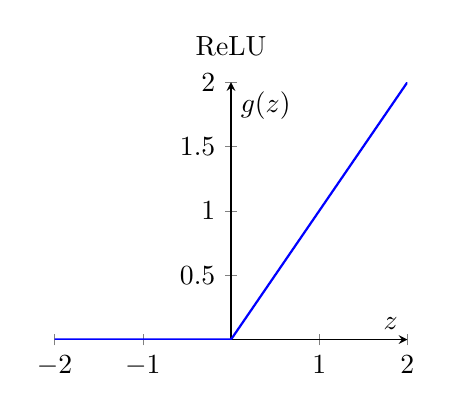
\begin{tikzpicture}
			      \begin{axis}[
					      axis lines=middle,
					      xlabel=$z$,
					      ylabel={$g(z)$},
					      title={ReLU},
					      width=0.5\textwidth,
					      height=0.4\textwidth
				      ]
				      \addplot[domain=-2:2, samples=200, thick, blue] {max(0, x)};
			      \end{axis}
		      \end{tikzpicture}
		      \caption{Funkcja aktywacyjna ReLU.}
		      \label{fig:relu}
	      \end{figure}
	      }
	\item{
	      \textbf{Sigmoid:}
	      \[
		      g(z) = \frac{1}{1 + e^{-z}}.
	      \]
	      \begin{figure}[ht]
		      \centering
		      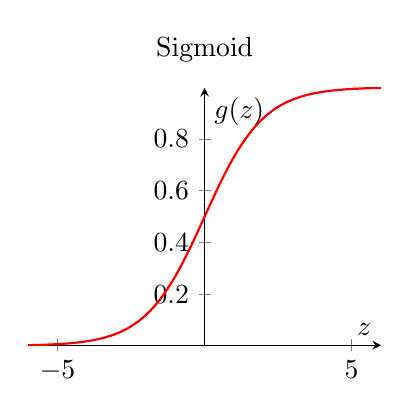
\begin{tikzpicture}
			      \begin{axis}[
					      axis lines=middle,
					      xlabel=$z$,
					      ylabel={$g(z)$},
					      title={Sigmoid},
					      width=0.5\textwidth,
					      height=0.4\textwidth
				      ]
				      \addplot[domain=-6:6, samples=200, thick, red] {1/(1 + exp(-x))};
			      \end{axis}
		      \end{tikzpicture}
		      \caption{Funkcja aktywacyjna Sigmoid.}
		      \label{fig:sigmoid}
	      \end{figure}
	      }
	\item {
	      \textbf{Tanh:}
	      \[
		      g(z) = \tanh(z) = \frac{e^z - e^{-z}}{e^z + e^{-z}}.
	      \]

	      \begin{figure}[ht]
		      \centering
		      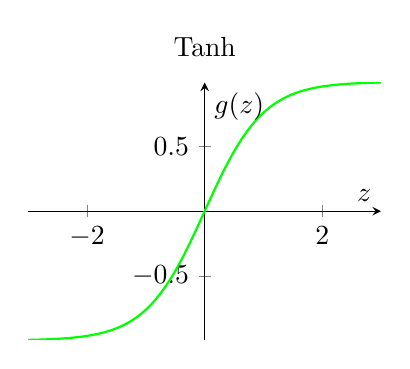
\begin{tikzpicture}
			      \begin{axis}[
					      axis lines=middle,
					      xlabel=$z$,
					      ylabel={$g(z)$},
					      title={Tanh},
					      width=0.5\textwidth,
					      height=0.4\textwidth
				      ]
				      \addplot[domain=-3:3, samples=200, thick, green] {tanh(x)};
			      \end{axis}
		      \end{tikzpicture}
		      \caption{Funkcja aktywacyjna Tanh.}
		      \label{fig:tanh}
	      \end{figure}
	      }
\end{itemize}

\paragraph{Wykresy funkcji aktywacyjnych:}

\subsubsection{Parametry modelu}

Parametry modelu (np. wagi \(w\) i biasy \(b\)) są wartościami liczbowymi, które model dostosowuje podczas procesu uczenia. Trenowanie modelu polega na minimalizacji funkcji kosztu (ang. loss function), która mierzy różnicę między przewidywaniami modelu a rzeczywistymi wartościami.

\[
	L = \frac{1}{n} \sum_{i=1}^{n} (y_i - \hat{y}_i)^2,
\]

gdzie \(y_i\) to rzeczywista wartość, a \(\hat{y}_i\) to przewidywana wartość modelu.

\subsection{Środowisko}
Środowisko jest otoczeniem, w którym agent działa. Dostarcza stanów \( S \), które opisują aktualną sytuację, oraz nagród \( R \), które oceniają jakość podjętych działań.

\subsection{Stan}
Stan opisuje bieżącą sytuację w środowisku, np. pozycję Mario w grze, liczbę żyć, czy stan przeszkód.

\subsection{Akcja}
Akcja to decyzja podjęta przez agenta, np. poruszanie się w lewo, w prawo, skok, czy bieganie.

\subsection{Nagroda}
Nagroda to liczba, którą agent otrzymuje za podjęcie akcji w danym stanie. Odpowiedni dobór nagród jest kluczowy dla skuteczności algorytmu:
\begin{itemize}
	\item \textbf{Pozytywne nagrody} motywują do osiągania celów,
	\item \textbf{Kary} odstraszają od niepożądanych działań.
\end{itemize}

Przykładowo w grze Super Mario Bros nagroda może być przyznawana za:
\begin{itemize}
	\item Zabicie przeciwnika,
	\item Przejście na kolejny poziom,
	\item Utratę życia (kara).
\end{itemize}
\begin{figure}[ht]
	\begin{center}
		\resizebox{\textwidth}{!}{
			\begin{tikzpicture}[
					node distance=2.5cm, % Odstęp między węzłami
					align=center, % Wyśrodkowanie tekstu w węzłach
					>=latex, % Strzałki w stylu LaTeX
					%every node/.style={draw, text width=3cm} % Styl węzłów
				]

				\node[rectangle, minimum width=5cm, draw=black] (full_frame) {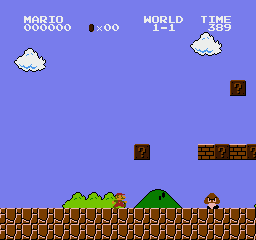
\includegraphics[width=4cm]{img/full_frame.png}\\Obraz generowany przez emulator NES};

				\node[right of=full_frame, xshift=6cm, draw=black] (compressed_frame) {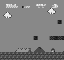
\includegraphics[width=2.5cm]{img/compressed_frame.png} \\Skompresowany obraz};
				\node (model) [right of=compressed_frame, draw = black, minimum height=2cm, xshift=2cm] {Model};
				\node (controller) [right of=model, draw=black, minimum height = 2cm, xshift=1cm, minimum width = 2cm] {Przyciski\\kontrolera\\NES};

				\draw[<-] (compressed_frame.west) -- (full_frame.east) node[midway] {Zmniejszenie\\ rozmiaru \\ konwersja na skalę \\szarości};
				\draw[<-] (model.west) -- (compressed_frame.east) node[midway]{Konwersja\\na tensor};
				\draw[<-] (controller.west) -- (model.east) node[midway] {Predykcja\\wciśnięć};

			\end{tikzpicture}
		}
	\end{center}
	\caption{Ogólny schemat działania programu}
	\label{fig:sys_diagram}
\end{figure}
